\documentclass[10pt,a4paper]{article}
\usepackage[latin1]{inputenc}
\usepackage{amsmath}
\usepackage{amsfonts}
\usepackage{amssymb}
\usepackage{graphicx}
\usepackage{multicol}
\usepackage{changepage}
\usepackage{float}
\usepackage{cite}
\usepackage{url}
\usepackage{imakeidx}
\makeindex

\usepackage[left=2.50cm, right=2.50cm]{geometry}
\usepackage[spanish]{babel}

\author{Axel}
\title{Portada siempre practica}

\begin{document}
%encabezado 
\pagestyle{plain}{
\pagestyle{empty}
\changepage{3cm}{1cm}{-0.5cm}{-0.5cm}{}{-2cm}{}{}{}
\noindent

%sEGIUN EL formato de sus imagenes, deben encontrar una configuracion adeacuada para ustedes
{\small
\begin{tabular}{p{0.626\textwidth} p{0.50\textwidth} }

\includegraphics[scale=0.26]{uaem.jpg} &  
\includegraphics[scale=0.3]{ico.jpg}
\end{tabular}
}

%datos de la caratula
\begin{center}
\par\vspace{2cm} %Rspacoo dejado antes del encabezado
{
\Huge\textbf{
Universidad Aut\'onoma del Estado de Mex\'ico \\[1cm] Ingenieria en Computaci\'on
}
}
\par\vspace{1.5cm}
{
\Large\textbf{ Materia: Redes Neuronales
}
}
\par\vspace{1.5cm}
{
\large\textbf{Axel Valenzuela Ju\'arez \\ 12 de Octubre del 2019  } 
}
\par\vspace{1.5cm}

\end{center}
\clearpage

}

\printindex

\section{
Perceptr\'on Simple
}
\paragraph{Se necesita comprender el funcionamiento del perceptr\'on simple para empezar a programar, as\'i que el primer paso fue revisar las presentaciones que nos proporcion\'o el profesor. Un perceptr\'on simple recibe 2 entradas, un vector de entrada y una vector de salida. Fig: \ref{fig:Eperceptron}}

\begin{figure}[h]
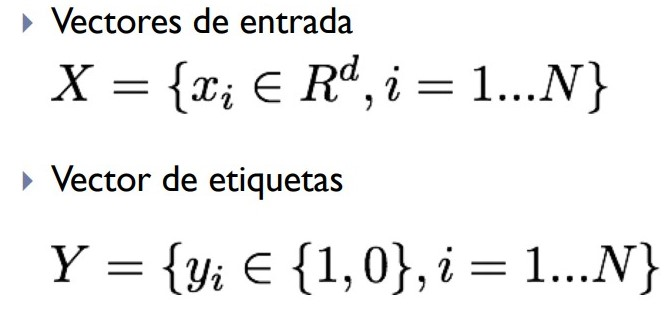
\includegraphics[scale=0.4] {Eperceptron.jpg}
\caption{Entradas del Perceptr\'on.}
\label{fig:Eperceptron}
\end{figure}

\paragraph{Para aplicar el perceptr\'on es necesario determinar los vectores de W, un perceptr\'on recibe dos entradas y un vector w para as\'i obtener una salida, se puede ver la representaci\'on de un perceptr\'on a continuaci\'on. Fig: \ref{fig:Rperceptron} }

\begin{figure}[h]
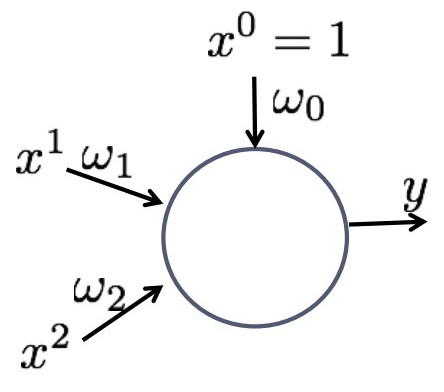
\includegraphics[scale=0.4] {RepPerc.jpg}
\caption{Representaci\'on de un perceptr\'on.}
\label{fig:Rperceptron}
\end{figure}

\paragraph{Para predecir la respuesta del perceptr\'on se ocupa la siguiente formula. Fig: \ref{fig:Formula}}

\begin{figure}[h]
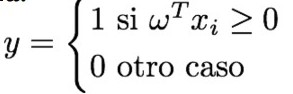
\includegraphics[scale=0.5] {f.jpg}
\caption{Pormula para predecir el resultado de un perceptr\'on.}
\label{fig:Formula}
\end{figure}

\paragraph{El algoritmo que ocupa el perceptr\'on es muy simple ya que se compone de dos for y un if y su respectivo else, se multiplica el vector W por el vector X, para poder multiplicarlos se necesita sacar la transpuesta de W, y despu\'es simplemente se compara el resultado, si el resultado es mayor que 0 se le asigna el valor de 1 a $"y"$ y si es menor se le asigna un 0.}

\paragraph{Lo interesante del algoritmo es la \'ultima parte ya que en esta es donde se decide la frontera de decisi\'on m\'as optima a base de los resultados de Y, el algoritmo est\'a hecho para que la frontera de decisi\'on se mueva seg\'un m\'as convenga hasta obtener un resultado \'optimo. Fig: \ref{fig:Algo} }

\begin{figure}[h]
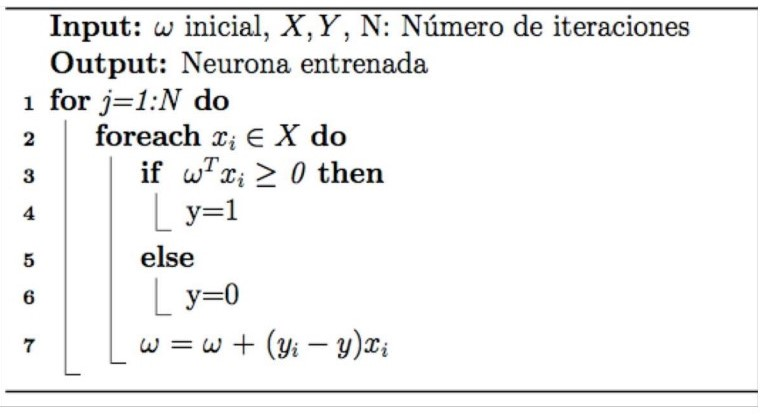
\includegraphics[scale=0.5] {Algorit.jpg}
\caption{Algoritmo para implementar el Perceptr\'on Simple.}
\label{fig:Algo}
\end{figure}

\section{
Codificaci\'on
}

\paragraph{El Primer paso en mi caso fue leer los datos de prueba, sacar los datos de la clase para tenerlos disponibles ya que se ocupan m\'as adelante en el algoritmo. Tambi\'en separe los datos que en este caso serian X (x1,x2) para posteriormente agregarle una columna con n\'umeros 1. }

\paragraph{Como siguiente paso cont\'e las columnas que exist\'ian esto para que el programa tenga la opci\'on de funcionar independientemente de la cantidad de datos que se metan, el siguiente paso que decid\'i hacer fue crear N n\'umeros aleatorios para el vector de W, en este caso fueron 3, ya que es el n\'umero de columnas m\'as 1 e inmediatamente saque la transpuesta de W ya que as\'i lo dicta el algoritmo. Fig: \ref{fig:CreacionW} }
\begin{figure}[h]
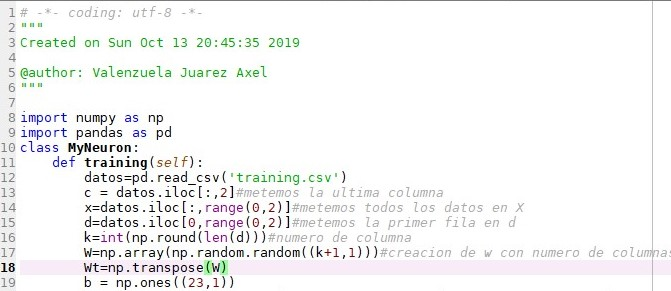
\includegraphics[scale=0.5] {cod1.jpg}
\caption{Primer fragmento de codigo.}
\label{fig:CreacionW}
\end{figure}

\paragraph{Cree una matriz de n\'umeros 1, para agregarse a los datos X y la agregue con la instrucci\'on append. Despu\'es de realizar esto empec\'e a crear el algoritmo como lo muestra la Fig: \ref{fig:Algo} }

\paragraph{Se multiplica el vector W por el vector X con el resultado se compara en un if si es mayor a 0 se le asignara el valor de 1 a Y, si es menor a 0 se le asignara un 0 a Y. Esto se realiza por cada fila que contenga X, al final el algoritmo corrige a W aument\'andole o rest\'andole valores.}

\paragraph{Una vez que obtuve el mejor valor de W lo mande a otra funci\'on para aplicarlo a los datos de test, para hacerlo utilice lo que ya hab\'ia hecho antes, leer el archivo, obtener el total de filas y aumentar una columna de unos. Multiplique a W por el vector de X de los datos de testing, y simplemente imprim\'i a Y como lo muestra la Fig: \ref{fig:testing}}
\begin{figure}[h]
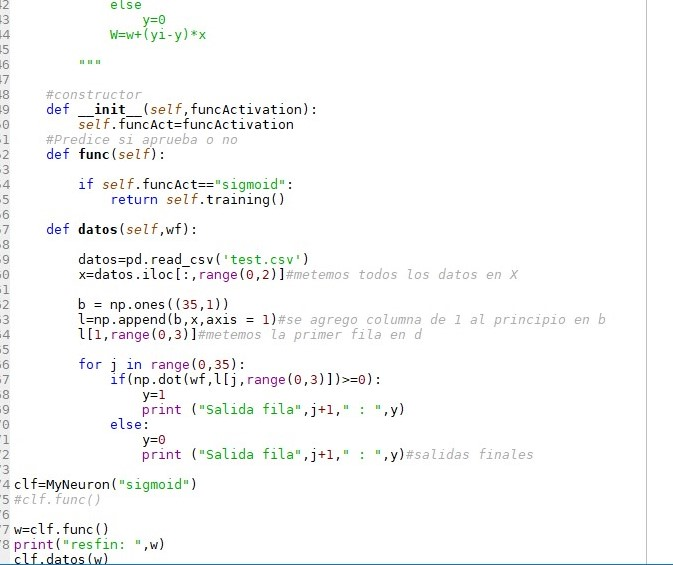
\includegraphics[scale=0.4] {cod2.jpg}
\caption{Uso de W para los datos de testing.}
\label{fig:testing}
\end{figure}

\paragraph{Para finalizar ejecute el programa y compare los resultados, los cuales se pueden observar en la Fig: \ref{fig:Res} }

\begin{figure}[h]
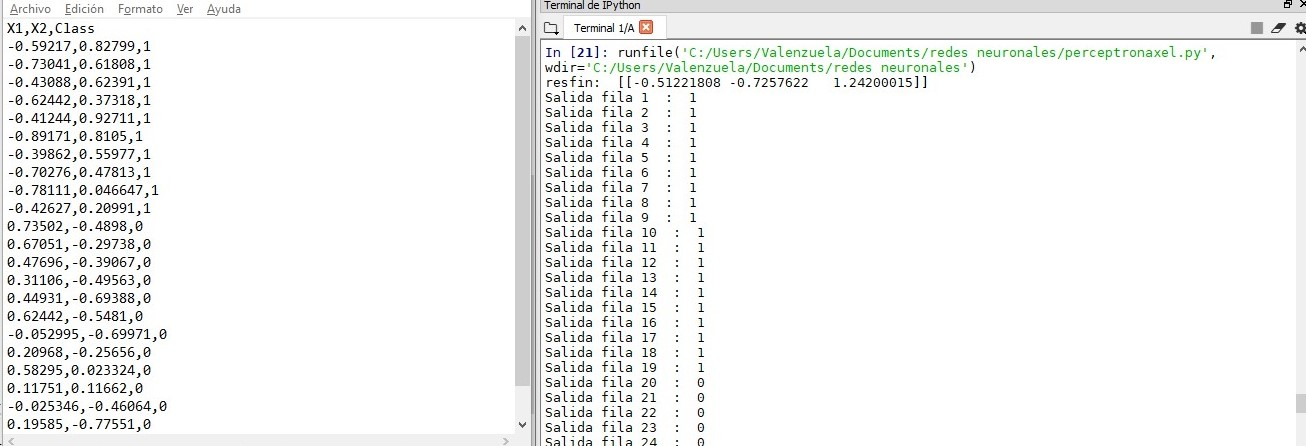
\includegraphics[scale=0.4] {res.jpg}
\caption{Comparaci\'on del Resultado de la Ejecuci\'on del Programa.}
\label{fig:Res}
\end{figure}

\section{Conclusion}
\paragraph{El perceptr\'on simple nos muestra como algo tan simple logra un gran resultado, espec\'ificamente en lograr obtener la mejor frontera de decisi\'on para un caso en particular, esto permite tener m\'as autonom\'ia ya que no se adivina ni se calcula por otra persona. En conclusi\'on el perceptr\'on simple es un gran comienzo a la hora de adentrarnos a las redes neuronales, es simple, efectivo y demuestra que a veces menos es m\'as.}

\section{Referencias}
\paragraph{Kumar, N. (14 de Octubre de 2019). hackernoon.com. Obtenido de 
$https://hackernoon.com/implementing-the-perceptron-algorithm-from-scratch-in-python-48be2d07b1c0$
}

\paragraph{CHAU, L . A.2019.El perceptr\'on. Zumpango: INGENIER\'IA EN COMPUTACI\'ON.}

\end{document}